

In the rest of this thesis, we present our approaches that contribute to achieve our goal of automatically testing code generators and tuning compilers. Figure \ref{fig:overview} depicts an overview of how the different contributions we propose are connected to each other and how they contribute to address the challenges of the state of the art, described earlier.

\begin{figure}[h]
	\center
	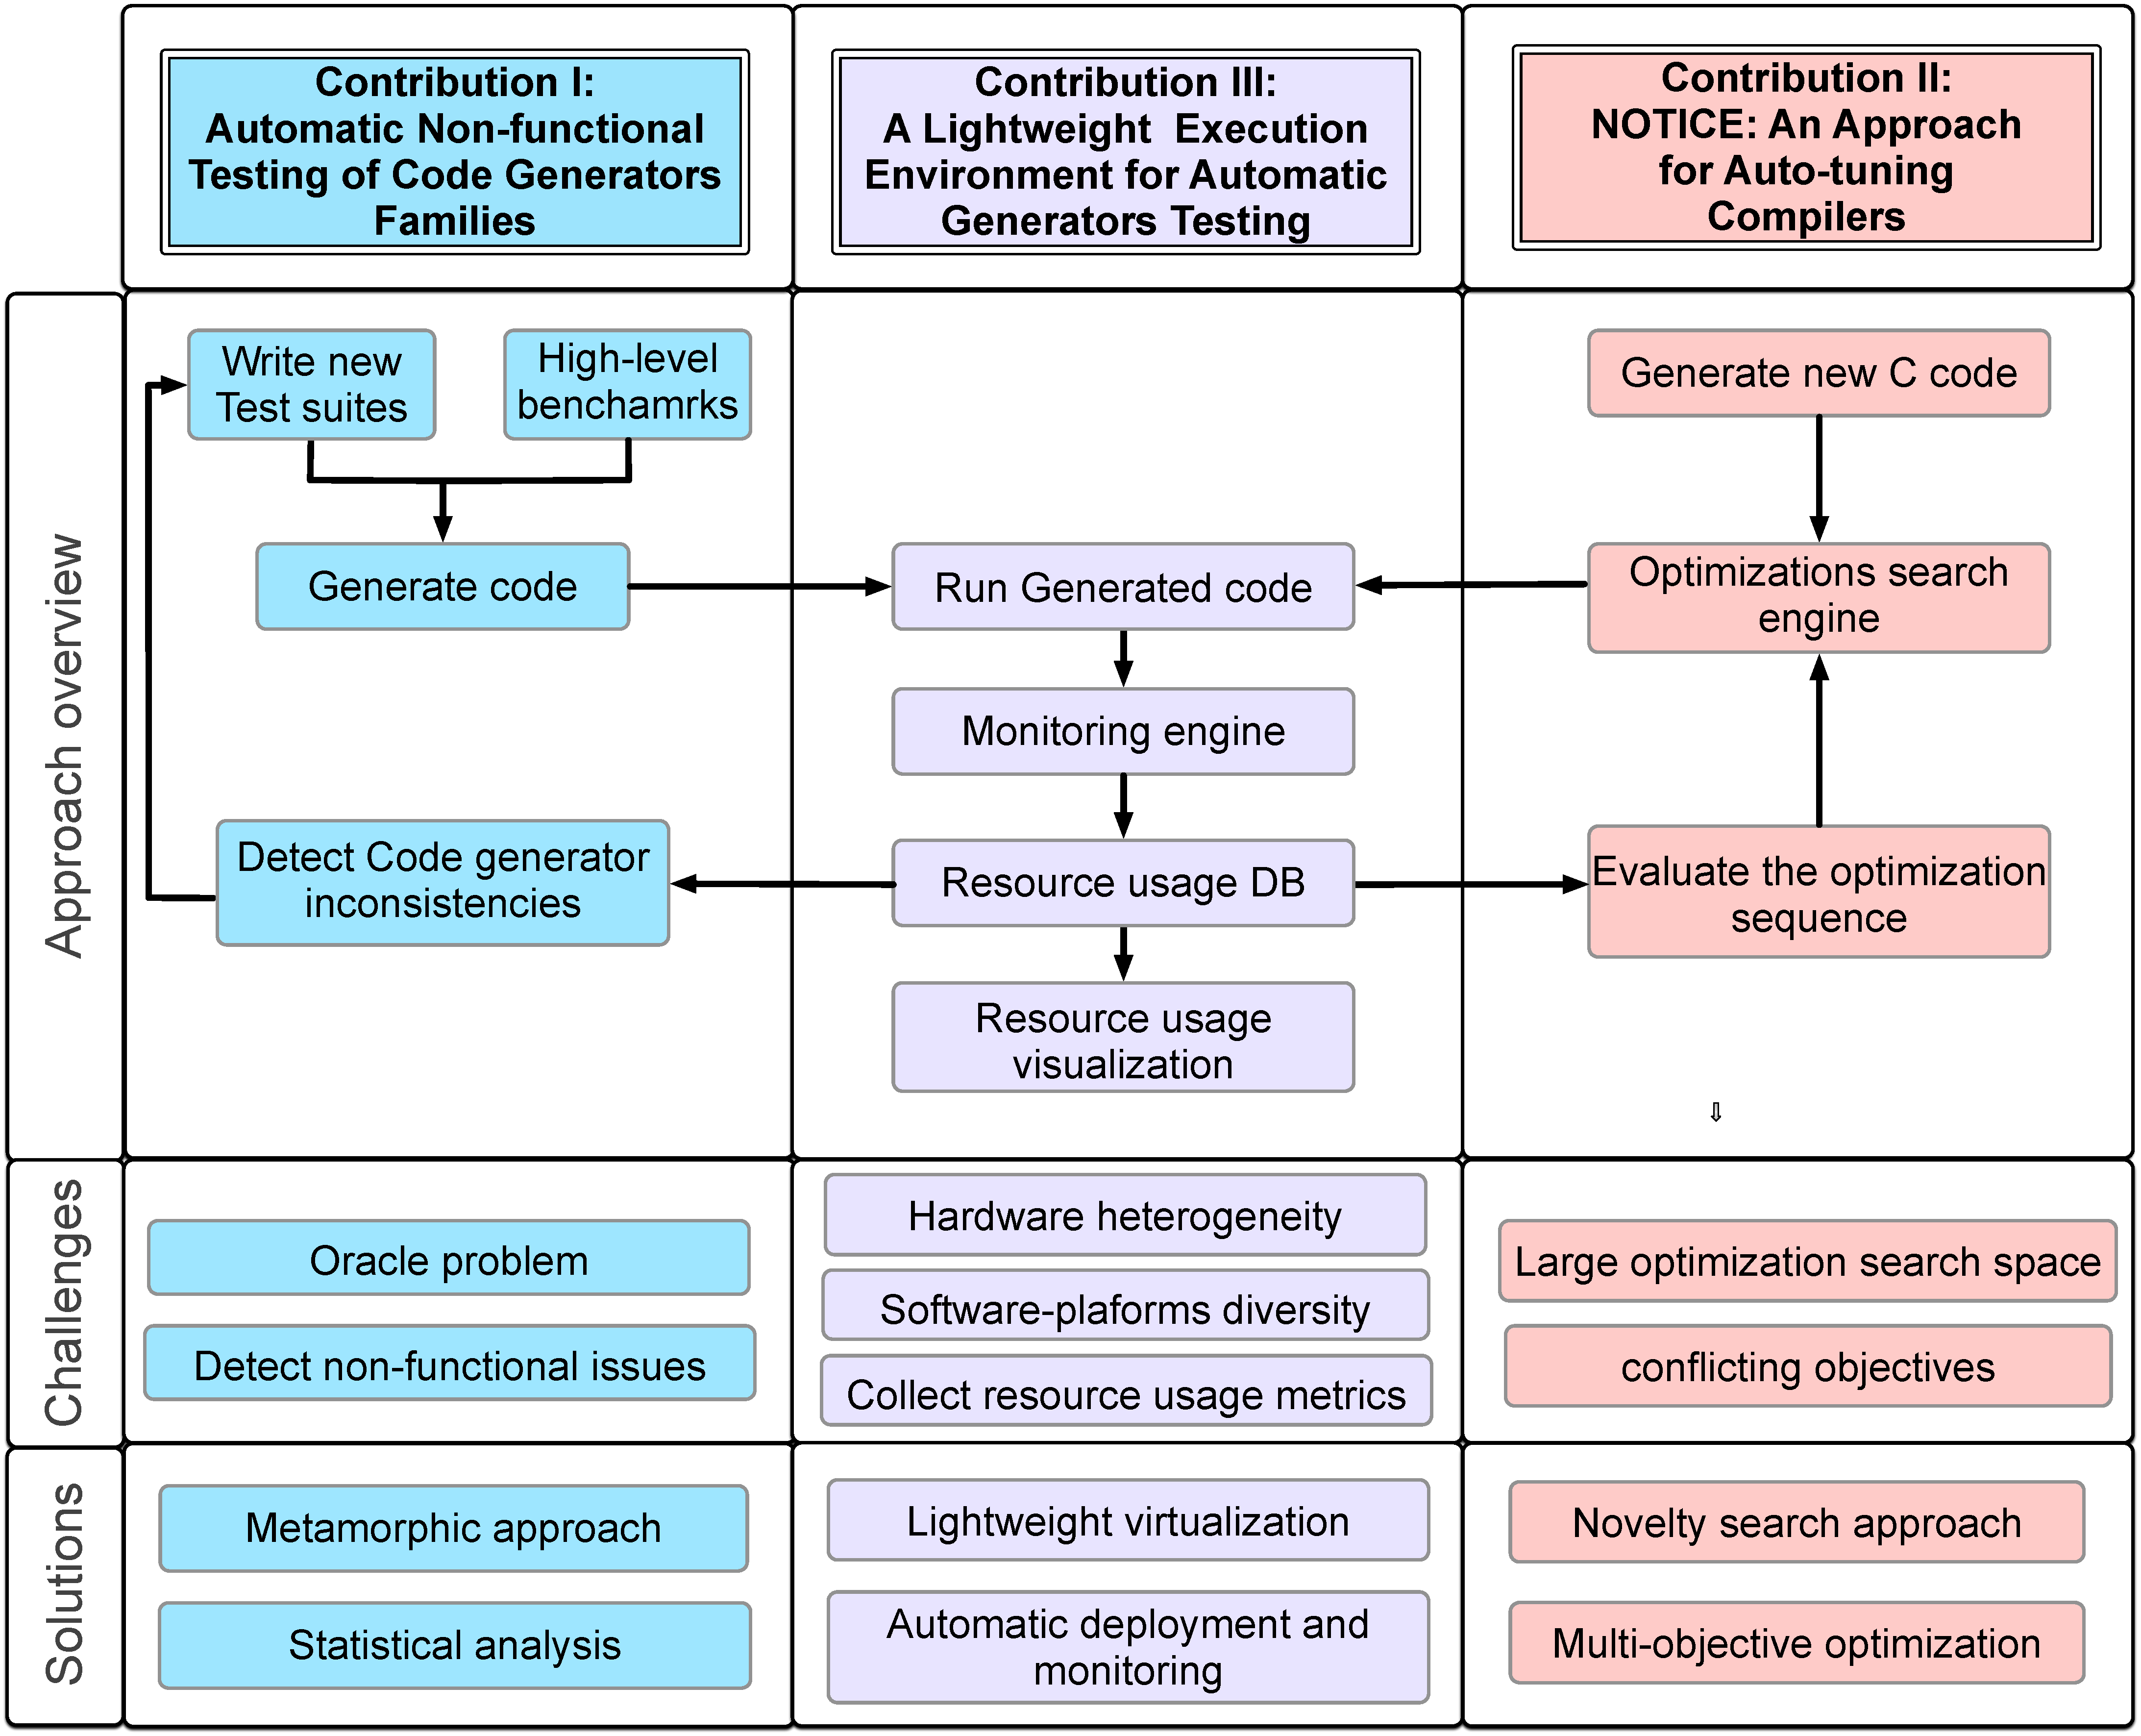
\includegraphics[scale=0.23]{Chapitre0/fig/overview}
	\caption{Summary of contributions}
	\label{fig:overview}
\end{figure}

This thesis makes three main contributions:
\begin{itemize}
	\item \textbf{Contribution I: Automatic non-functional testing of code generators families (in blue): }
	
	In this contribution (Chapter \ref{chap:code generators}), we propose an approach for automatic non-functional  testing of code generators. As discussed earlier, existing solutions lack of automation and efficiency to find code generator issues. Particularly, the problem of non-functional testing as well as the test oracle definition are not addressed. In this contribution, we address the limitations of the state of the art by describing an approach based on metamorphic testing and statistical analysis to efficiently detect inconsistencies within code generator families.
	Thus, starting from high-level benchmarks and test suites, we generate automatically source code to five different target languages (i.e. using a code generator family). We execute the generated code and evaluate the resource usage metrics using the lightweight testing infrastructure presented in the contribution III. Inconsistencies are then reported for further inspection.  
	
	\item \textbf{Contribution II: NOTICE, An approach for auto-tuning compilers (in red):}
	
	As discussed in the state of the art, there are two main limitations we would address: the problem of exploring the large optimization search space and the multi-objective exploration for finding trade-offs between conflicting objectives. 
	Thus, we present in Chapter \ref{chap:compilers}, an adaptation of the novelty search algorithm for compilers auto-tuning. Our contribution focuses on tuning GCC compilers based on randomly generated C programs.
	This approach shares the same monitoring infrastructure as the previous contribution in order to evaluate the impact of discovered optimization sequences on resource usage. The outcome of this approach is the best set of optimizations sequences for a giving hardware architecture, for a given input program and for a specific resource usage metric. We also provide a multi-objective optimization evaluation to tackle the problem of conflicting objectives.
	
	\item \textbf{Contribution III: A lightweight execution environment for software testing and monitoring (in purple):}
	
	We propose in Chapter \ref{chap:docker}, a common infrastructure used by both previous contributions to automate software testing and monitoring. Particularly, it serves as a lightweight execution environment to mimic real software and hardware settings, required to run the generated code. It is based on micro-services namely Docker in order to automate the software deployment, execution and monitoring. It is used by the first both contributions to provide information about the quality of the generated code in terms of memory and CPU usage. Finally, we provide in this contribution a mechanism to visualize at runtime the resource usage of running programs. This contribution address the limitations of the state of the art, namely the lack of solutions that handle the software and hardware requirements when testing/tuning generators.
\end{itemize}

The validation of each contribution is presented in the corresponding chapter. Different experiments are used to illustrate the characteristics of each solution we present.



